% chapters/glitch.tex
%
% Copyright 2023 Alexander Lyttle.
%
% This work may be distributed and/or modified under the conditions of the
% LaTeX Project Public License (LPPL) version 1.3 or later.
%
% The latest version of this license is in
% https://www.latex-project.org/lppl.txt and version 1.3 or later is part of
% all distributions of LaTeX version 2005/12/01 or later.
%
%
\chapter[Acoustic glitches]{Acoustic glitches as a signature of helium abundance}\label{chap:glitch}

A glitch arises from a sharp structural variation in the star.

Explain that glitches can be a signature of helium abundance. If we can model the glitch consistently between models and observed stars, we can add parameters to the HBM which contain information about helium.

In this chapter, we explore the theoretical background of acoustic glitches

\section[1D example]{A one-dimensional example of a glitch}\label{sec:1d-glitch}

A rapid variation in the structure of a medium induces an oscillation (\(\delta\omega\)) in the eigenfrequencies. To demonstrate this, we will explore a simple one-dimensional example \citep[e.g][]{Verner2005}. Consider a medium bound from \(x=0\) to \(x=L\) in which pressure waves can propagate at constant speed \(c\). The longitudinal displacement of the wave \(\xi\) must obey the wave equation,
%
\begin{equation}
    \frac{\partial^2\xi(x, t)}{\partial t^2} = c^2 \frac{\partial^2\xi(x, t)}{\partial x^2},
\end{equation}
%
at a given position \(x\) and time \(t\). A general solution to the wave may be written as a sum of right- and left-travelling waves. In terms of the angular frequency \(\omega\), wave number \(k\), and complex coefficients \((A, B)\),
%
\begin{equation}
    \xi(x, t) = A e^{i (\omega t - k x)} + B e^{i (\omega t + k x)},
\end{equation}
%
where \(\omega\) and \(k\) satisfy \(\omega = c k\). Solving for the boundary condition \(\xi(0, t) = 0\) we find \(B = - A\). Substituting Euler's formula, \(A = (r/2) e^{i\phi}\), we can write the real solution for \(\xi\) as,
%
\begin{equation}
    \real\left[\xi(x, t)\right] = r \sin k x \sin(\omega t + \phi),
\end{equation}
%
representing the physical component of the wave, where \(r\) and \(\phi\) are the amplitude and temporal phase respectively. Solutions for \(\omega\) which satisfy \(\xi(L, t)=0\) may then be found,
%
\begin{equation}
    \omega_n = c \frac{n \pi}{L}, \label{eq:omega-n}
\end{equation}
%
where \(n\) is a non-zero integer (the \(n=0\) solution would give \(\xi=0\) everywhere).

Now, let us suppose there is a small structural perturbation (or glitch) in the medium at position \(x_0\) with half-width \(\delta x\). Figure \ref{fig:1d-diagram} shows this system divided into 3 regions, with region 2 containing the glitch. In region 2, the speed of sound is \(c + \delta c\) and the corresponding wave number is \(k + \delta k\). We want to find the frequencies which correspond to standing waves in this system and compare them to that of the homogeneous medium above. We will show that the resulting eigenfrequencies oscillate with an amplitude and period that relates to the properties of the glitch.

Firstly, we propose solutions to the wave for each region by considering reflection and transmission at each boundary. Initially ignoring the wave superposed by a reflection at \(x=L\),
%
\begin{align}
    \xi_1(x, t) &= e^{i(\omega t - k x)} + A e^{i(\omega t + k x)}, \label{eq:xi1-r} \\
    \xi_2(x, t) &= Be^{i(\omega t - (k + \delta k) x)} + C e^{i(\omega t + (k + \delta k) x)}, \label{eq:xi2-r} \\
    \xi_3(x, t) &= D e^{i(\omega t - k x)}, \label{eq:xi3-r}
\end{align}
%
where complex coefficients \(A\) and \(C\) represent reflections, and \(B\) and \(D\) represent transmissions, at \(x_0 \pm \delta x\) respectively. Later, we will substitute the left-travelling wave (\(- \xi\{-k, -\delta k\}\)) after determining the values of the coefficients.

\begin{figure}
    \centering
    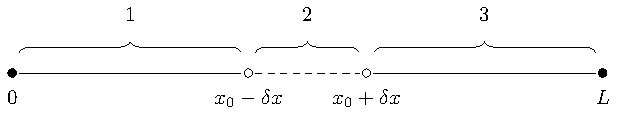
\includegraphics{figures/glitch-1d-example-diagram.pdf}
    \caption[A diagram showing a one-dimensional medium with a small structural perturbation.]{A diagram showing a one-dimensional medium split into three regions. 1: Fixed at \(x=0\) with a constant speed of sound \(c\); 2: A small structural perturbation centred at \(x=x_0\) with width \(2\delta x\) and constant speed of sound \(c + \delta c\); 3: Fixed at \(x=L\) with a constant speed of sound \(c\).}
    \label{fig:1d-diagram}
\end{figure}

The boundary conditions for this system are found by enforcing spacial continuity at \(x - \delta x\) and \(x + \delta x\),
%
\begin{align*}
    \xi_1(x_0 - \delta x, t) &= \xi_2(x_0 - \delta x, t), \\
    \xi_2(x_0 + \delta x, t) &= \xi_3(x_0 + \delta x, t), \\
    \frac{\partial \xi_1}{\partial x}(x_0 - \delta x, t) &= \frac{\partial \xi_2}{\partial x}(x_0 - \delta x, t), \\
    \frac{\partial \xi_2}{\partial x}(x_0 + \delta x, t) &= \frac{\partial \xi_3}{\partial x}(x_0 + \delta x, t).
\end{align*}
%
Solving these simultaneously with the Python package \textsc{sympy} gives the following equations for the complex coefficients\footnote{The code for these derivations are available at \url{\gitremote/tree/\gitbranch/notebooks}},
%
\begin{align}
    A &= \delta k (2k + \delta k) (1 - e^{4i \delta x (k + \delta k)}) e^{- 2i k (x_0 - \delta x)} \alpha^{-1}, \\
    B &= 2 k (2k + \delta k) e^{4i \delta x (k + \delta k)} e^{i \delta k (x_0 - \delta x)} \alpha^{-1}, \\
    C &= 2 k \delta k e^{- i (x_0 - \delta x) (2k + \delta k)} \alpha^{-1}, \\
    D &= 4 k (k + \delta k) e^{2 i \delta x (2k + \delta k)} \alpha^{-1},
\end{align}
%
where,
\begin{equation}
    \alpha = (2k + \delta k)^2 e^{4 i \delta x (k + \delta k)} - \delta k^2.
\end{equation}
%

Now we have solutions for the coefficients, we can superpose the right-travelling wave, \(\xi\{k, \delta k\} \rightarrow - \xi\{-k, -\delta k\}\) to get the full solution for the wave function. Substituting \(k \rightarrow -k\) and \(\delta k \rightarrow -\delta k\) into the coefficients yields their complex conjugates, \((\overline{A},\overline{B},\overline{C},\overline{D})\). This allows us to rewrite the wave functions into a more flexible form. For example, substituting Euler's formula, \(A = (r_A/2) e^{i\phi_A}\) and \(\overline{A} = (r_A/2) e^{-i\phi_A}\), Equation \ref{eq:xi1-r} now becomes,
%
\begin{equation}
    \xi_1(x, t) = e^{i \omega t} \left[ \frac{r_A}{2} \left( e^{i(kx + \phi_A)} - e^{-i(kx + \phi_A)} \right) - \left( e^{ikx} - e^{-ikx} \right) \right] \label{eq:xi1}
\end{equation}
%
where its real component is,
\begin{equation}
    \real\left[\xi_1(x, t)\right] = \sin \omega t \left[2 \sin kx - r_A \sin(kx + \phi_A)\right].
\end{equation}
%
However, this does not satisfy the boundary condition that the displacement is always zero at \(x=0\); \(\xi_1(0, t) = - r_A \sin \omega t \sin(\phi_A) \neq 0\). To do so, we introduce a small displacement phase \(\epsilon\) caused by the glitch, and let \(x \rightarrow x + \epsilon\). We will determine \(\epsilon\) shortly. In the meantime, superposing the right-travelling wave and substituting Euler's formula into Equations \ref{eq:xi2-r} and \ref{eq:xi3-r}, we can write the real components of the wave functions,
%
% \begin{align}
%     \xi_3(x, t) = \frac{r_A}{2} e^{i \omega t} \left[ e^{i(k(x + \epsilon) + \phi_A)} - e^{-i(k(x + \epsilon) + \phi_A)} \right],
% \end{align}
%
% with a real solution in trigonometric form,
%
\begin{align}
    \real[\xi_1(x, t)] &= \sin \omega t \left\{2 \sin[k (x + \epsilon)] - r_A \sin[k(x + \epsilon) - \phi_A]\right\} \label{eq:xi1-real} \\
    \real[\xi_2(x, t)] &= \sin \omega t \left\{ r_B \sin[(k + \delta k)(x + \epsilon) - \phi_B] - r_C \sin[(k + \delta k)(x + \epsilon) - \phi_C]\right\} \\
    \real[\xi_3(x, t)] &= \sin \omega t \left\{r_D \sin[k(x + \epsilon) - \phi_D]\right\} \label{eq:xi3-real}
\end{align}
%
Imposing the boundary condition \(\xi_1(0, t) = 0\), we solve Equation \ref{eq:xi1-real} for \(\epsilon\) at \(x=0\),
%
\begin{align}
    \epsilon &= \frac{1}{k} \tan^{-1}\left( \frac{(r_A / 2) \sin(\phi_A)}{1 - (r_A/2) \cos(\phi_A)} \right), \notag\\
    &= \frac{1}{k} \tan^{-1}\left( \frac{\imag[A]}{1 - \real[A]} \right). \label{eq:1d-phase}
\end{align}
%

Finally, we can impose the boundary condition \(\xi_3(L, t) = 0\) to solve for \(\omega\). Setting Equation \ref{eq:xi3-real} to zero, we can rewrite it in terms of the real and imaginary components of \(D\),
%
\begin{align}
    \sin \omega t \left\{r_D \sin[k(L + \epsilon) - \phi_D]\right\} &= 0, \quad (\div \sin \omega t) \notag \\
    r_D \cos \phi_D \sin[k(L + \epsilon)] - r_D \sin \phi_D \cos[k(L + \epsilon)] &= 0, \notag \\
    \real[D] \sin[k(L + \epsilon)] - \imag[D] \cos[k(L + \epsilon)] &=0. \label{eq:1d-glitch-sol}
\end{align}
%
The glitch affects the amplitude and phase of the wave, because if we set \(\epsilon = 0\) and \(D = 1\) we recover the homogeneous frequency solutions (Equation \ref{eq:omega-n}). Unfortunately, solving Equation \ref{eq:1d-glitch-sol} for \(\omega\) is not possible analytically. However, we can find individual roots (or modes, \(\omega_n\)) numerically.

We find \(\omega_n\) by solving Equation \ref{eq:1d-glitch-sol} using Newton's method for \(n = 1,\dots,50\), with \(c=1\), \(L=1\), and several values of \(x_0\), \(\delta x\), and \(\delta c\). Initial guesses are obtained from the homogeneous medium solutions (\(\omega_n^0\)) in Equation \ref{eq:omega-n}. The difference between the solutions for \(\omega_n\) and those from the homogeneous medium, \(\delta \omega_n = \omega_n - \omega_n^0\), are shown in Figure \ref{fig:1d-results}. We can see an oscillation in \(\delta\omega\) induced by the glitch. Physically, this arises from the change in phase \(\epsilon\) caused as the wave travels through the glitch region. As the nodes pass in and out of the region with changing \(n\), the sensitivity of the wave to the glitch oscillates. The form of \(\delta\omega\) appears to have a linear component and a short period oscillation modulated by a longer period. As the location of the glitch (\(x_0\)) increases towards the edge of the system, the short-period oscillation of \(\delta\omega\) increases. Similarly, as the the half-width of the glitch (\(\delta x\)) increases, the longer modulation period increases. Furthermore, an increasing change in sound speed (\(\delta c\)) increases the amplitude of \(\delta\omega\). Finally, increasing both \(\delta x\) and \(\delta c\) increases the slope of \(\delta\omega\).

\begin{figure}
    \centering
    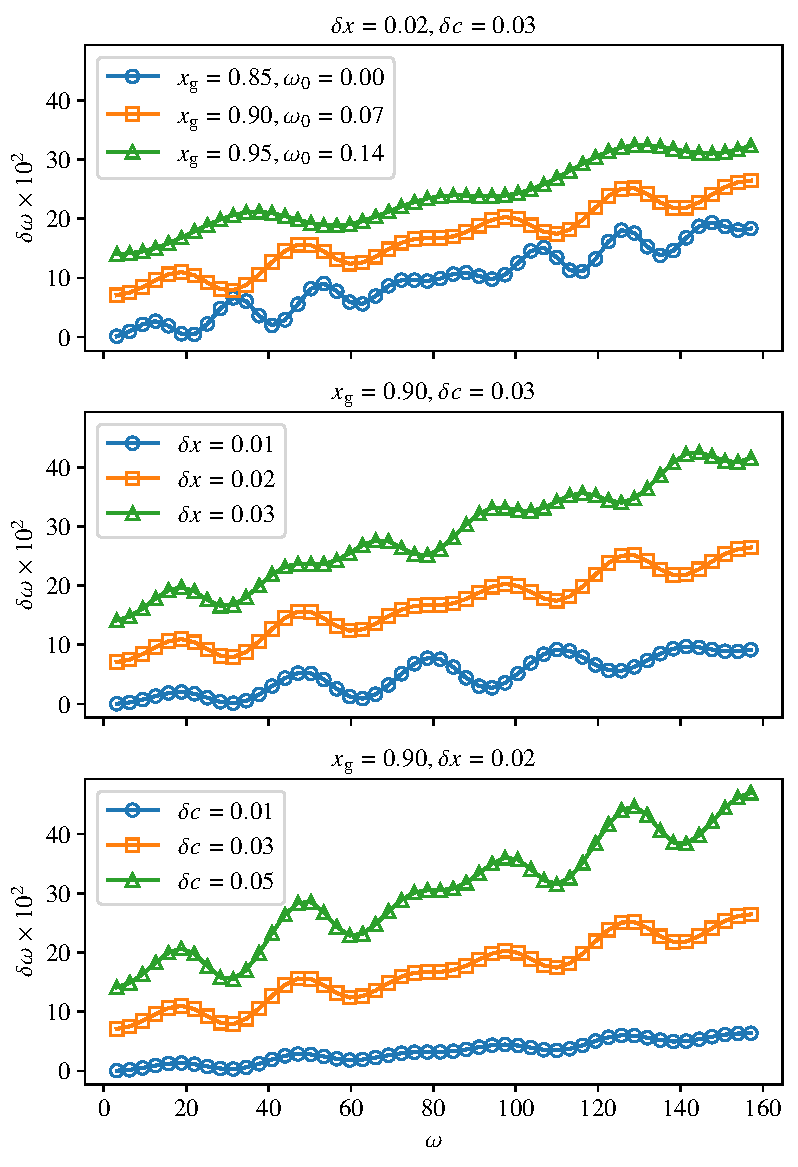
\includegraphics{figures/glitch-1d-example-results.pdf}
    \caption{The change in mode frequency induced by a change in sound speed of \(\delta c\) from \(x_0 - \delta x\) to \(x_0 + \delta x\) in a one-dimensional medium, bound such that \(x \in [0, 1]\) (see Figure \ref{fig:1d-diagram}). Outside of the perturbation the speed of sound, \(c=1\).
    The frequencies in the top panel are offset by \(\omega_0\).
    Points are joined by straight lines to guide the eye.
    }
    \label{fig:1d-results}
\end{figure}


%This may be interpreted as the nodes of each standing wave passing in and out of region 2 with increasing \(n\). Where there is a node, the wave is least sensitive to a change in structure, and 

The small phase offset \(\epsilon\) in Equation \ref{eq:1d-phase} is required for the wave function to satisfy the boundary conditions at \(x = 0\). However, adding \(\epsilon\) shifts the effective location of \(x_0\). We plot \(\epsilon\) against \(\omega\) in Figure \ref{fig:1d-phase} and show that its magnitude is \(\sim 10^{-4}\), much smaller than the location and size of region 2. The oscillation caused by the glitch also shows up in Figure \ref{fig:1d-phase}, with its properties affected in a similar way to Figure \ref{fig:1d-results}.

\begin{figure}
    \centering
    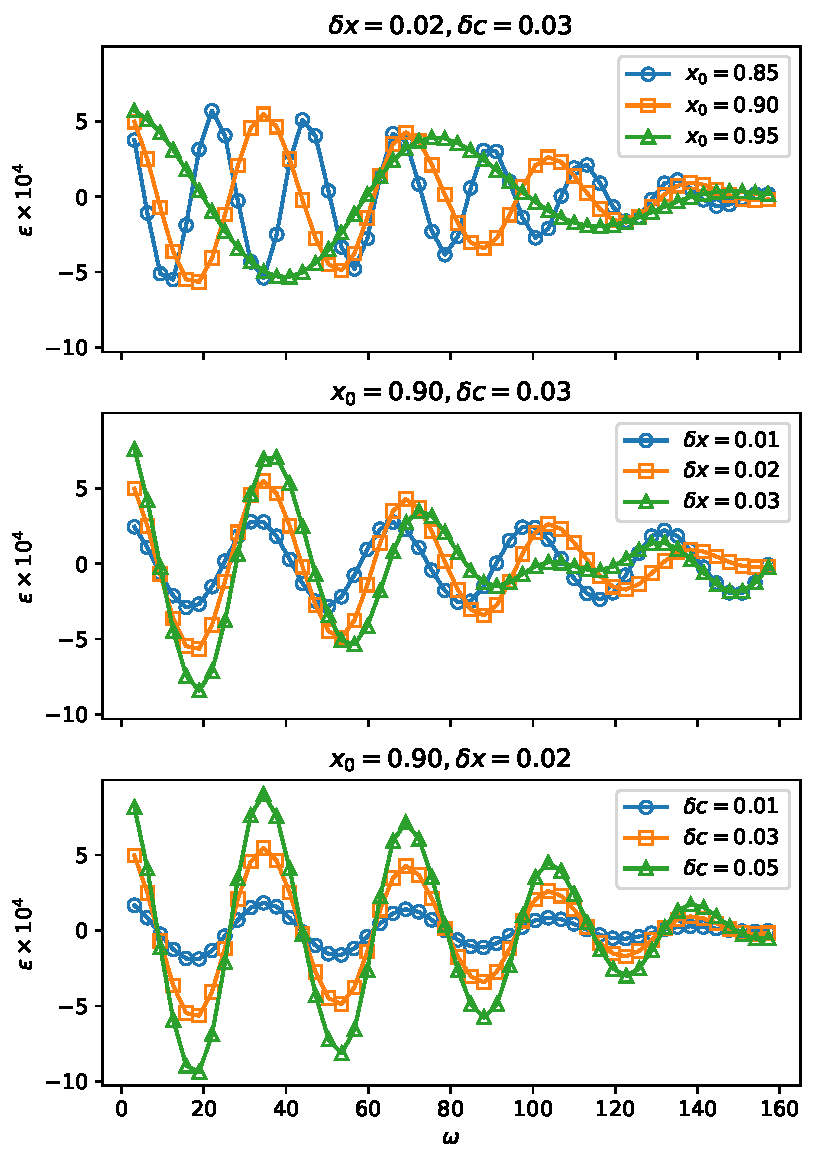
\includegraphics{figures/glitch-1d-example-phase.pdf}
    \caption{The same as Figure \ref{fig:1d-results} but showing the phase offset \(\epsilon\) required to satisfy the boundary conditions.}
    \label{fig:1d-phase}
\end{figure}

Finding an approximate solution for \(\delta\omega\) is beyond the scope of this simple example. However, we can show that by modelling \(\delta\omega\), we can recover information about the structural glitch. Let us build a model \(\delta\omega = f(\omega)\). Looking at Figure \ref{fig:1d-results}, we propose a form for \(f\),
%
\begin{equation}
    f(\omega) = a_1 \omega - a_2 \sin (\tau_1 \omega) \cos (\tau_2 \omega), \label{eq:1d-domega-func}
\end{equation}
%
where \(a_1\) and \(a_2\) are coefficients which are both functions of \(\delta x\) and \(\delta c\). Parameters \(\tau_1\) and \(\tau_2\) are the `frequencies' (units of time\footnote{A frequency in \(\omega\) would have units of time, but shouldn't be confused with a periodicity in \(\omega\).}) of oscillations in \(\delta\omega\), which are functions of \(\delta x\) and \(x_0\) respectively.

We fit Equation \ref{eq:1d-domega-func} to \(\delta\omega_n\) obtained from a glitch located at \(x_0 = 0.9\), with half-width \(\delta x = 0.02\), and change in sound speed \(\delta c = 0.03\). The best fitting line is shown in Figure \ref{fig:1d-fit}. Repeating this for different glitch parameters, it can be shown empirically how the `frequencies' \(\tau_1\) and \(\tau_2\) relate to the half-width and location of the glitch respectively. It emerges that \(\tau_1 \approx 2\delta\tau\), where \(\delta\tau\) is half the acoustic width of the glitch (i.e. the time at which sound takes to transverse the region). The second `frequency' \(\tau_2 \approx 2\tau_0\), where \(\tau_0\) is the acoustic depth from the nearest edge to the centre of the glitch, \(x_0\),
%
\begin{equation}
    \tau_0 = \int_0^{x_0'} \frac{\dd x}{c(x)},
\end{equation}
%
where \(x_0' = L/2 - | L/2 - x_0 |\) is the relative location of the glitch from the nearest edge of the system. Since the speed of sound \(c(x) \approx 1\) throughout the medium, \(x_0 \approx L - \tau_0\). Our example fit yields \(\tau_1 \approx \SI{0.0389}{\second\per\radian}\) and \(\tau_2 \approx \SI{0.199}{\second\per\radian}\), approximately recovering the input glitch half-width of \num{0.02} and location of \num{0.9}.

% NOTE: Could take this further to show a1 = 2 dc dtau / L and a2 = dc / L

\begin{figure}
    \centering
    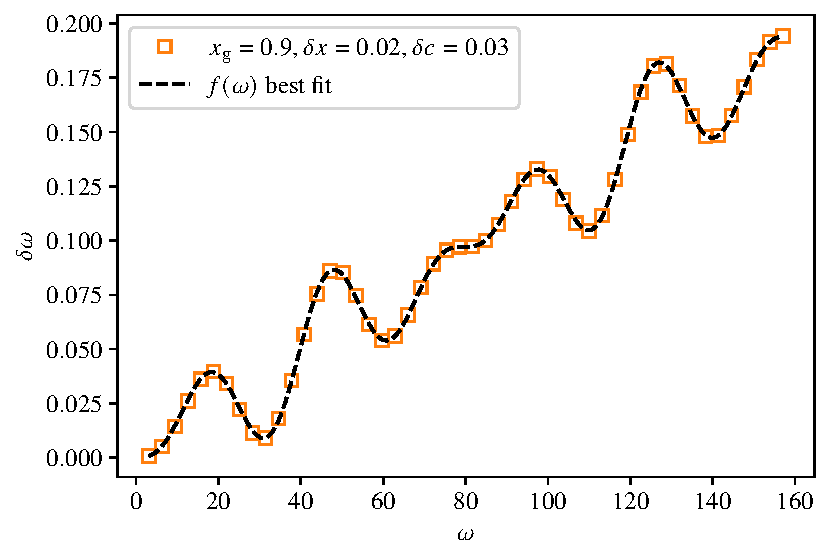
\includegraphics{figures/glitch-1d-fit.pdf}
    \caption{Best fit of Equation \ref{eq:1d-domega-func} to \(\delta\omega_n\) for \(n=1,\dots,50\), \(L=1\), and \(c=1\).}
    \label{fig:1d-fit}
\end{figure}

It would not be hard to believe that a similar oscillation could be found in the mode frequencies of a star, although its structure is more complicated. We showed that fitting to \(\delta\omega\) we may can recover properties of a glitch. In the next section, we will explore glitches in stars.

% NOTES: Go slowly through this. The next step is to fit a simple mode to theses oscillations and show that we can find x0 and dx. And show how the amplitude scales with dc.

% NOTES: When it comes to fitting the helium glitch, consider first fitting a GP to the modes with a free noise term. Fix the kernel scale to a series of values and show that we can see the glitch in the residuals. Of course, this leaves the question of what kernel scale to use. Well, we could just model everything at once!

\section{Acoustic glitches in stars}

In the previous section, we considered a glitch in a homogeneous medium, where the speed of sound is constant everywhere else. In a star, the adiabatic sound speed is not constant. It depends on the density (\(\rho\)) and pressure (\(P\)),
%
\begin{equation}
    c^2 = \gamma \frac{P}{\rho},
\end{equation}
%
where \(\gamma \equiv \Gamma_1\) is the first adiabatic exponent,
%
\begin{equation}
    \gamma = \left( \frac{\partial \ln P}{\partial \ln \rho} \right)_S,
\end{equation}
%
at constant entropy, \(S\). Chandrasekhar \needcite{} introduced three adiabatic exponents (\(\Gamma_1,\Gamma_2,\Gamma_3\)) to describe the non-ideal gas inside a star. In this chapter, we do not use the other two and hence refer the first as \(\gamma\).

For the most part, \(\gamma\), \(P\), and \(\rho\) change smoothly with radius inside a star. However, a small structural glitch in these quantities would lead to a sudden change in sound speed. We have seen how such a perturbation can lead to an oscillation in the eigenfrequencies of pressure waves in a homogeneous medium. Characterising this oscillation allows us to measure the properties of the glitch. If similar glitches were present in a star, then we might be able to do the same. In this section, we explore the origins of glitches inside a Sun-like star. Then, we see what effect these have on the eigenfrequencies, a quantity we can measure through asteroseismology.

Firstly, let us look at the sound speed profile of a Sun-like star. Particularly, we want to see how the sound speed changes on the timescale of a pressure wave moving through the star. As discovered in Section \ref{sec:1d-glitch}, a convenient timescale to work with is the acoustic depth, \(\tau\). For a star, we define \(\tau_\star\) as the time taken for a pressure wave to travel from its surface (\(r=R\)) to some radius \(r_\star\),
%
\begin{equation}
    \tau(r_\star) = \int_R^{r_\star} \frac{\dd r}{c(r)}.
\end{equation}
%
The acoustic radius of the star, \(\Tau = \tau(R)\) relates approximately to the average large frequency spacing \(\langle\Delta\nu\rangle^{-1} \approx 2T_0\).

In Figure \ref{fig:sound-speed-gradient}, we show the sound speed gradient with respect to \(\tau\) for model S. We see how the speed of sound changes smoothly throughout the star. In the convective envelope, there is a noticeable wiggle around \SI{700}{\second} and a sharp discontinuity at its base. The first is caused by the ionisation of helium, which affects \(\gamma\) by increasing the number of free electrons and thus modifying the free energy of the gas. We explore this further in Section \ref{sec:helium-glitch}. The second is due to a change in the temperature gradient as the structure moves from convectively unstable to radiative, which will be discussed in Section \ref{sec:bcz-glitch} \todo{Put a few references here of work which has studied these before}.

\begin{figure}
    \centering
    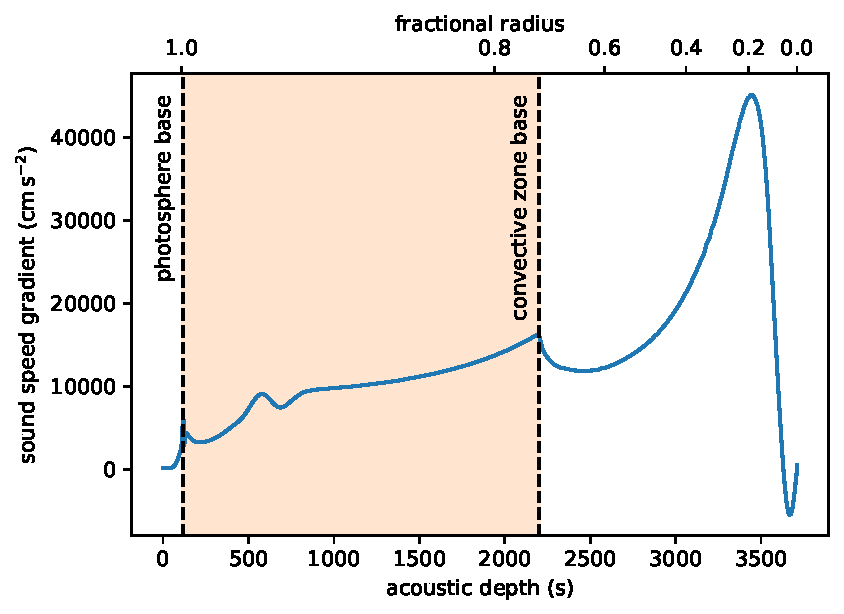
\includegraphics{figures/sound-speed-gradient.pdf}
    \caption{The sound speed gradient (\(\dd c/\dd \tau\)) of model S with respect to the acoustic depth (\(\tau\)). The fractional radius to the photosphere base is given on the top axis. The convective envelope is shaded and the bases of the photosphere and convective zone are marked with dashed lines.}
    \label{fig:sound-speed-gradient}
\end{figure}

\subsection{Helium ionisation glitch}\label{sec:helium-glitch}

The pressure-density gradient at constant entropy for an ideal monatomic gas, \(\gamma = 5/3\). However, as a species ionises, its chemical potential changes, modifying the free energy of the gas and thus inducing a depression in \(\gamma\) \todo{Improve and verify this explaination}. Using an approximate form for the first adiabatic exponent from \citet{Houdayer.Reese.ea2021}, we show how \(\gamma\) is affected by the ionisation of helium and hydrogen in Figure \ref{fig:gamma-zones}. We see that hydrogen ionisation has the largest effect on \(\gamma\) close to the surface of the star. The first and second ionisations of helium occurs deeper in the star, at higher temperatures. We can see that the second ionisation of helium has a greater affect on \(\gamma\) than the first. This is because the ionisation energy of He II is higher than He I and the ground state degeneracy of He II is less than He I \todo{We know from equations but why physically}.

\begin{figure}
    \centering
    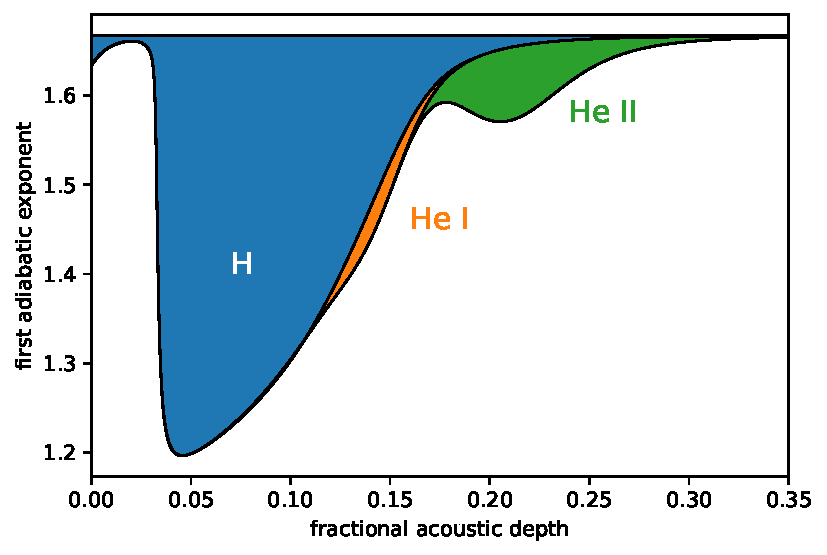
\includegraphics{figures/adiabatic-ionisation-regions.pdf}
    \caption{The depressions in the first adiabatic exponent (\(\gamma\)) caused by the ionisation of hydrogen (H), and the first and second ionisations of helium (He I and He II). The x-axis is the fractional acoustic depth from the surface of the star, \(\tau/\Tau\).}
    \label{fig:gamma-zones}
\end{figure}

Lets consider a star of mass \(M\) with hydrogen and helium mass fractions of \(X\) and \(Y\) respectively. To demonstrate the effect of ionisation and stellar structure on \(\gamma\) we can use a recent... \citet{Houdayer.Reese.ea2021} approximated \(\gamma\) in a solar-like star as a function of temperature and density,
%
\begin{equation}
    \gamma \approx \frac{5}{3} - \frac{2}{3} \, \eta(T, \rho), \label{eq:gamma1}
\end{equation}
%
where \(\eta\) represents the depression in \(\gamma\). Considering a hydrogen-helium mixture where \(X + Y \approx 1\), \(\eta\) is given by,
%
\begin{equation}
    \begin{split}
        \eta(T, \rho) &= \frac{1}{\partial_{TT}^2 f} \left[n_\hydrogen y_\hydrogen \, (1 - y_\hydrogen) \, \frac{(\chi_\hydrogen / k_B T)^2}{2 - y_\hydrogen}
        % \right. \\ &\left. 
        + n_\helium y_\helium^{(1)} \left(1 - y_\helium^{(1)}\right) \left(\frac{\chi_\helium^{(1)}}{k_B T}\right)^2 
        \right. \\ &\left.
        + \, n_\helium y_\helium^{(2)} \left(1 - y_\helium^{(2)}\right) \left(\frac{\chi_\helium^{(2)}}{k_B T}\right)^2\right],
    \end{split}
\end{equation}
%
where \(k_B\) is the Boltzmann constant. The parameter \(\partial_{TT}^2\) is the second partial derivative of the free energy density with respect to \(T\),
%
\begin{equation}
    \begin{split}
        \partial_{TT}^2 f &\approx \frac{3}{2} + n_\hydrogen y_\hydrogen \left[ \frac{3}{2} + \frac{(1 - y_\hydrogen)}{2 - y_\hydrogen} \left(\frac{3}{2} + \frac{\chi_\hydrogen}{k_B T}\right)^2 \right] %\\
        + n_\helium y_\helium^{(1)} \left[ \frac{3}{2} + \left(1 - y_\helium^{(1)}\right) \left(\frac{3}{2} + \frac{\chi_\helium^{(1)}}{k_B T}\right)^2 \right] \\
        &+ n_\helium y_\helium^{(2)} \left[ \frac{3}{2} + \left(1 - y_\helium^{(2)}\right) \left(\frac{3}{2} + \frac{\chi_\helium^{(2)}}{k_B T}\right)^2 \right],
    \end{split}
\end{equation}
%
where \(n_\mathbb{X} = N_\mathbb{X} / N\) is the number density and \(\chi_\mathbb{X}^{i}\) is the \(i\)-th ionisation energy of species \(\mathbb{X}\). Parameter \(y_\mathbb{X}^i\) is related to a reduced form of Saha's equation \needcite,
%
\begin{equation}
    \frac{(y_\mathbb{X}^i)^q}{1 - y_\mathbb{X}^i} = \frac{2 g_\mathbb{X}^i}{g_\mathbb{X}^{i-1}} \frac{\overline{m}}{\rho \lambda_e^3} \, e^{- \chi_\mathbb{X}^i / k_B T},
\end{equation}
%
where \(q = 2\) for hydrogen, \(q = 1\) for helium, \(\overline{m} = M/N\) is the mean mass, and \(g_\mathbb{X}^i\) is the ground-state degeneracy of ionisation state \(i\). 

\begin{figure}
    \centering
    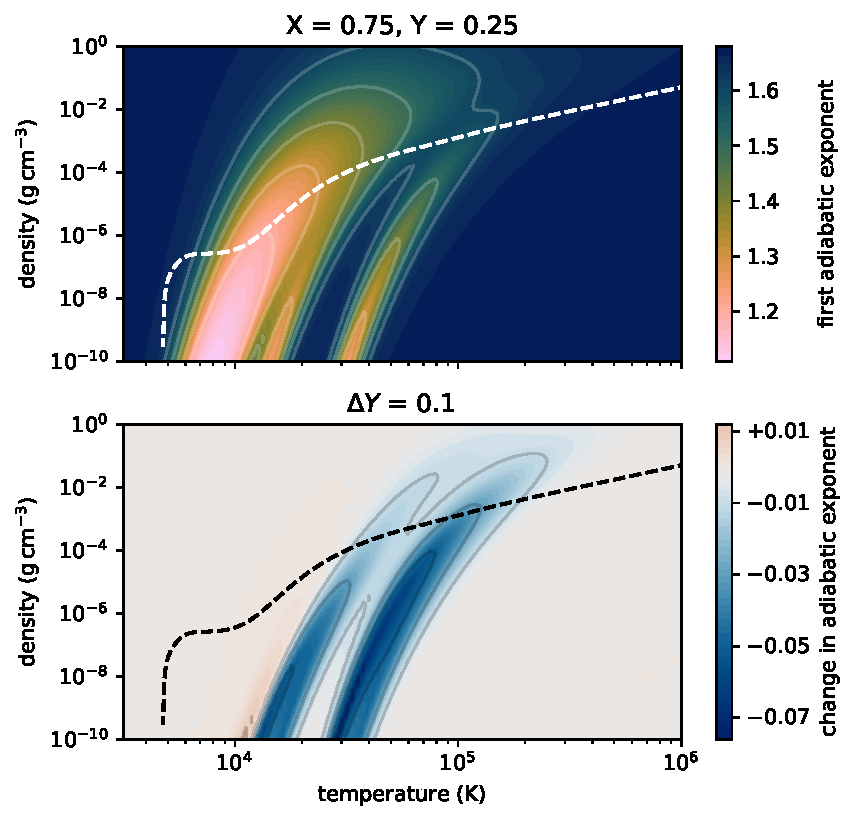
\includegraphics{figures/adiabatic-ionisation-temp.pdf}
    \caption{Temperature-density profile of a Sun-like star. \emph{Top:} The first adiabatic exponent \(\gamma\) as a function of temperature and density, calculated using Equation \ref{eq:gamma1} for a helium mass fraction, \(Y=0.25\). \emph{Bottom:} The change in \(\gamma\) induced by a change in helium abundance, \(\Delta Y = 0.1\). In both panels, the dashed line shows the temperature-density profile of model S.}
    \label{fig:gamma-temp-density}
\end{figure}

\begin{figure}
    \centering
    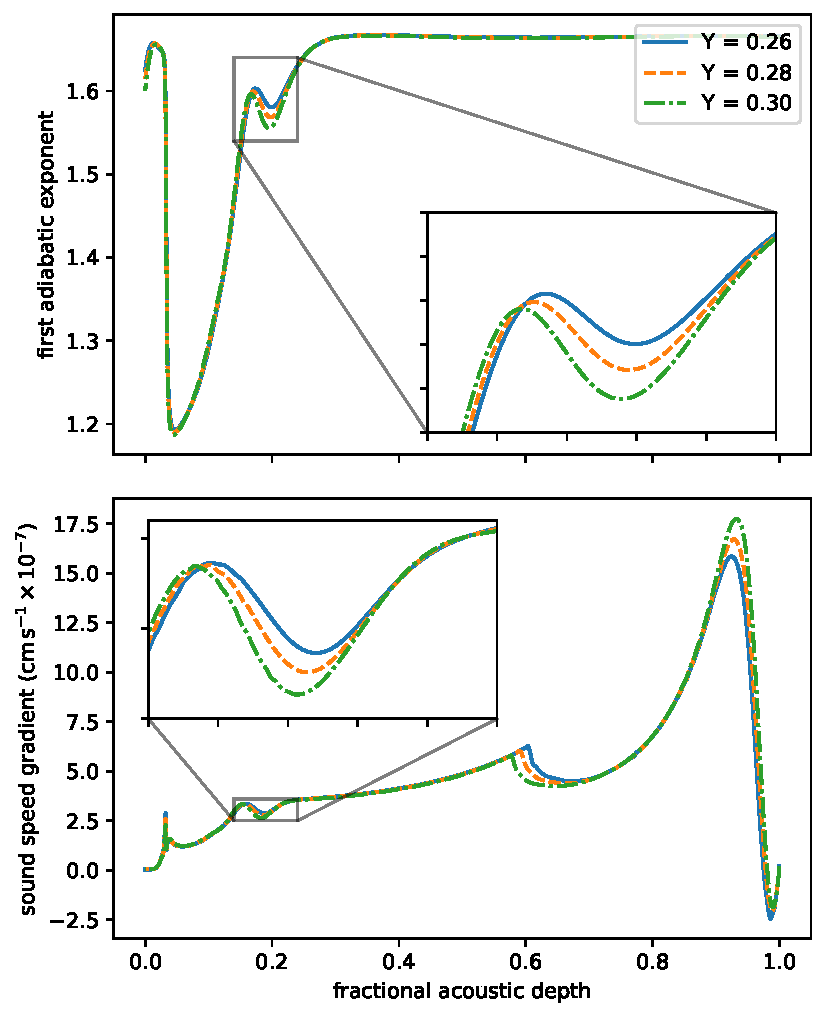
\includegraphics{figures/helium-ionisation-sound-speed.pdf}
    \caption{The effect on the sound speed profile for three solar-like stars with initial helium mass fractions of 0.26 (\emph{solid}), 0.28 (\emph{dashed}), and 0.3 (\emph{dot-dashed}). The models were each evolved to a central helium mass fraction of 0.6. \emph{Top:} The first adiabatic exponent \(gamma\). \emph{Bottom:} The sound speed gradient \(\dd c/\dd t\) where \(t = \tau/T_0\) is the fractional acoustic depth (plot on the x-axis).}
    \label{fig:gamma-sound-speed}
\end{figure}

\todo{Now we look at the radial order kernels and how they are sensitive to different region}

\begin{itemize}
    \color{red}
    \item Use variational principle to link modes to change in structure
    \item Introduce kernels to plot and show mode sensitivity
    \item Go from kernels to the form of \(\delta\nu\) from Houdek and Gough
\end{itemize}

From the variational principle \citep{Chandrasekhar1939,Chandrasekhar1964}, we can write the characteristic frequencies for a spherically symmetric, slowly rotating star,
%
\begin{equation}
    \omega^2 = \frac{\mathcal{E}}{\mathcal{I}}\label{eq:var-prin}
\end{equation}
%
where \(\mathcal{I}\) is the mode inertia,
%
\begin{equation}
    \mathcal{I} = \int_0^R \vect{\xi} \cdot \vect{\xi} \rho r^2 \dd r
\end{equation}
%
and \(\mathcal{E}\) is proportional to its energy,
%
\begin{equation}
    \mathcal{E} = \int_0^R \left[\gamma P (\dive{\vect{\xi}})^2 + 2(\vect{\xi}\cdot \nabla P) \dive{\vect{\xi}} + (\vect{\xi}\cdot \nabla P) (\vect{\xi}\cdot\nabla\ln\rho)\right] r^2 \dd r
\end{equation}
%
where \(\vect{\xi}\) is the Lagrangian perturbation vector of the pulsation mode. \todo{Explain the meaning of each term}. A structural glitch in the star would cause a small change in frequency (\(\delta\omega\)). Differentiating both sides of Equation \ref{eq:var-prin} with respect to \(\omega\), we get,
%
\begin{align}
    2\omega &= \frac{1}{\mathcal{I}} \left( \frac{\delta\mathcal{E}}{\delta\omega} - \omega^2 \frac{\delta\mathcal{I}}{\delta\omega}\right), \qquad \left[\times \frac{\delta\omega}{2\omega^2}\right] \notag \\
    \frac{\delta\omega}{\omega} &= \frac{1}{2\,\mathcal{I}} \left(\frac{\delta\mathcal{E}}{\omega^2} - \delta\mathcal{I}\right).
\end{align}
%
To see the effect of a change in structure on the modes, it is possible to rewrite this as a function of the so-called structural kernels \(\mathcal{K}_{a,b}\), for example,
%
\begin{equation}
    \frac{\delta\omega}{\omega} = \int_0^R \left(\mathcal{K}_{c^2,\rho} \frac{\delta c^2}{c^2} + \mathcal{K}_{\rho,c^2} \frac{\delta \rho}{\rho} \right) \dd r.\label{eq:kernels}
\end{equation}
%
where \(\mathcal{K}_{a, b}\) gives the relative effect on \(\omega\) due to a perturbation in quantity \(a\) at fixed \(b\) at a given \(r\). These kernels are defined in \citet{Gough.Thompson1991}. We plot the kernels in Figure \ref{fig:kernels} for a few modes. Both decay through the star, meaning that the modes are less sensitive to structural changes deeper in the star. \todo{Explain why this is, from asymptotic theory frequencies determined by sound speed}. The second term of Equation \ref{eq:kernels} approximately integrates to zero, particularly for high-order modes. 

%
\begin{equation}
    \frac{\delta\omega}{\omega} \approx \int_0^R \mathcal{K}_{\gamma,\rho} \frac{\delta\gamma}{\gamma} \dd r,\label{eq:delta-omega}
\end{equation}
%
where \(\mathcal{K}_{\gamma,\rho} \equiv \mathcal{K}_{c^2,\rho}\) is shown in \citet{Gough1993} to satisfy,
%
\begin{equation}
    \omega^2 \mathcal{I}\mathcal{K}_{\gamma,\rho} = \frac12 \gamma P (\dive{\vect{\xi}})^2 r^2.\label{eq:gamma-kernel}
\end{equation}
%
show how this gets to, using equations for \(\xi_r\) and pressure perturbation \(P'\) from eq. 24-25 of e.g. \citet{Shibahashi1979}, \(\vect{\xi} = \xi_r \hat{r} + \vect{\xi}_h\) for high-order acoustic modes (where we can ignore the horizontal component of \(\vect{\xi}\)).
%
\begin{equation}
    \xi_r \approx \frac{\psi_0}{r}\sqrt{\frac{K}{\rho}} \cos\psi,\qquad
    (\dive{\vect{\xi}})^2 \approx \frac{\psi_0^2 \omega^3}{\gamma P c r^2} \sin^2\psi, \label{eq:xi-approx}
\end{equation}
%
where \(\psi_0\) is a proportionality constant and the radial wave number \(K \approx \omega / c\) for high-order acoustic modes. The phase term \(\psi \approx \omega \tau + \epsilon\) when \(\tau\) is not close to the upper turning point (where the wave is reflected near the stellar surface), and the small offset \(\epsilon\) is a slowly varying function of \(\tau\).

\begin{align}
    \mathcal{I} &\approx \int_0^R \xi_r^2 \rho r^2 \, \dd r \notag\\
    &\approx \psi_0^2 \int_0^R K \cos^2\psi \, \dd r \notag \\
    &= \frac12 \omega \psi_0^2 \int_0^R (1 + \cos 2 \psi) \frac{\dd r}{c}
\end{align}
%
Changing to an integral over acoustic depth we can evaluate it for high-order modes where \(\omega_n \ll T_0^{\,-1}\),
%
\begin{align}
    \mathcal{I} &\approx \frac12 \omega \psi_0^2 \int_0^{T_0} [1 + \cos 2 (\omega\tau + \epsilon)] \, \dd \tau \approx \frac12 \omega \psi_0^2 T_0.
\end{align}
%
Finally, substituting Equations \ref{eq:gamma-kernel} and \ref{eq:xi-approx} into Equation \ref{eq:delta-omega}, we get,
%
\begin{align}
    \frac{\delta\omega}{\omega} &\approx \frac{1}{2\omega^2\mathcal{I}} \int \delta\gamma P (\dive{\vect{\xi}})^2 r^2 \, \dd r, \notag \\
    &\approx \frac{\omega \psi_0^2}{2 \mathcal{I}} \int \frac{\delta\gamma}{\gamma}\sin^2\psi\frac{\dd r}{c}, \notag \\
    &= \frac{\omega \psi_0^2}{4 \mathcal{I}} \int \frac{\delta\gamma}{\gamma}(1 - \cos 2\psi)\frac{\dd r}{c}.
\end{align}
%
where the integral need only be evaluated in the region where \(\delta\gamma / \gamma\) is non-zero. We can see that \(\delta\omega\) is split into a smooth and an oscillating component. The smooth component may be treated later, but for now we focus on the oscillating part of \(\delta\omega\). Substituting for \(\mathcal{I}\) and \(\psi\), changing to an integral over acoustic depth, and switching to cyclic frequency we get,
%
\begin{equation}
    \left.\frac{\delta\nu}{\nu}\right|_\mathrm{osc} \approx - \nu_0 \int \frac{\delta\gamma}{\gamma} \cos 2 (2 \pi\nu\tau + \epsilon) \, \dd \tau,
\end{equation}
%
where \(\omega = 2\pi\nu\), and \(\nu_0 = (2 T_0)^{-1}\) is the inverse acoustic diameter of the star (approximately the average large frequency separation \(\langle \Delta \nu \rangle\)).

We have shown that a perturbation in \(\gamma\) can induce an oscillation in \(\nu\). The functional from of this oscillation depends on \(\delta\gamma/\gamma\). As shown in Figures \ref{fig:gamma-zones} and \ref{fig:gamma-temp-density}, the dominant perturbation due to a change in helium abundance is from the second ionisation of helium. There have been different attempts to approximate \(\delta\gamma/\gamma\,|_\heII\) in the literature, for example using a Dirac delta function or a triangular function \citep{Monteiro.Christensen-Dalsgaard.ea1994, Monteiro.Thompson2005}. In recent years, work modelling the glitch has used the formulation from \citet{Houdek.Gough2007} where the perturbation is modelled with a Gaussian shape,
%
\begin{equation}
    \left.\frac{\delta\gamma}{\gamma}\right|_\heII \approx - \frac{\Gamma_\heII}{\Delta_\heII \sqrt{2\pi}} \, e^{- \frac12{(\tau - \tau_\heII)^2}/{\Delta_\heII^2} },
\end{equation}
%
where \(\Gamma_\heII\) is the area, \(\Delta_\heII\) is the characteristic width, and \(\tau_\heII\) is the center of the ionisation region.

Combine the above two equations, asymptotically integrate about \(\tau = \tau_\heII\) using \textsc{WolframAlpha}, dropping second-order terms in \(\tau - \tau_\heII\) we get the following from for the glitch oscillation \citep[cf.][]{Houdek.Gough2007},
%
\begin{align}
    % \left.\frac{\delta\nu}{\nu}\right|_{\heII, \mathrm{osc}} &\approx \frac{\nu_0 \Gamma_\heII}{\Delta_\heII \sqrt{2\pi}} \int \exp\left[ - \frac{(\tau - \tau_\heII)^2}{2\Delta_\heII^2} \right] \cos(4 \pi \nu \tau + \phi) \, \dd \tau \notag \\
    \left.\frac{\delta\nu}{\nu}\right|_{\heII, \mathrm{osc}} &\approx \frac{\Gamma_\heII \nu_0}{\Delta_\heII \sqrt{2\pi}} \int e^{- \frac12{(\tau - \tau_\heII)^2}/{\Delta_\heII^2} } \cos 2 (2 \pi \nu \tau + \epsilon) \, \dd \tau \notag \\
    &\approx \frac12 \, {\Gamma_\heII \nu_0} \, e^{- 8 \pi^2 \Delta_\heII^2 \nu^2} \, \mathrm{erfi}\left(2\sqrt{2}\,\pi\Delta_\heII\nu\right) \sin(4 \pi \nu \tau_\heII + \phi_\heII) \notag\\
    &\approx A_\heII \nu \, e^{- 8 \pi^2 \Delta_\heII^2 \nu^2} \sin(4 \pi \nu \tau_\heII + \phi_\heII)
\end{align}
%
where we expanded the imaginary error function \(\mathrm{erfi}(z)\) around \(z=0\) and drop terms of order \(\mathcal{O}(z^3)\). Parameters \(A_\heII = 2 \sqrt{2\pi} \, \Gamma_\heII \Delta_\heII \nu_0\), and \(\phi_\heII = 2\epsilon_\heII\), where we assume \(\epsilon \approx \epsilon_\heII\) is constant over the glitch region.

Notice how this differs slightly from \citet{Houdek.Gough2007}, who appear to set the error function term to one.

\subsection{Base of the convective zone glitch}\label{sec:bcz-glitch}

Other glitches are present. Sharp structure variation

\begin{figure}
    \centering
    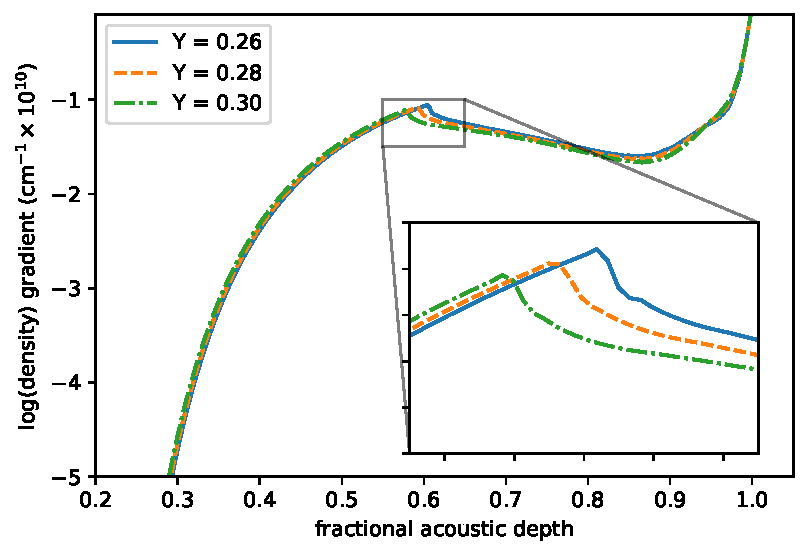
\includegraphics{figures/bcz-density-gradient.pdf}
    \caption{Discontinuity in the density gradient at the base of the convective zone for three solar-like stars with initial helium mass fractions of 0.26 (\emph{solid}), 0.28 (\emph{dashed}), and 0.3 (\emph{dot-dashed}).}
    \label{fig:bcz-density}
\end{figure}

\section[Modelling the glitch]{Modelling glitches in stellar oscillations}

One approach is in Houdek and Gough, to take a perturbation in gamma and propagate this to a perturbation in frequency.

\begin{itemize}
    \item Approx model for \(\delta\nu\)
    \item Need a smooth component
    \item Use Gaussian process to model smooth component
\end{itemize}

\subsection{Gaussian processes }\label{sec:glitch-gp}

